\section[Системное описание предметной области дипломного проекта]{%
  СИСТЕМНОЕ ОПИСАНИЕ ПРЕДМЕТНОЙ \\
  ОБЛАСТИ ДИПЛОМНОГО ПРОЕКТА
}\label{sec:spec}

Целью дипломной работы является проектирование и
разработка мобильного приложения, выполняющего отображение актуальной
финансовой информации, а именно: курсов валют в Республике Беларусь,
информации об отделениях банков с использованием сервисов геолокации,
возможность использования конвертера валют.

План-проспект проекта находится в приложении~A.


\subsection{Выбор программной платформы}

Для того, чтобы правильным образом выбрать программную платформу, обратимся к
общей тенденции развития рынка персональных компьютеров и мобильных устройств.

Так, уже в 2012 году мировой рынок персональных компьютеров начинает показывать спад:
в третьем квартале этого года наблюдается снижение объема
поставок техники на 8,6\% по сравнению с аналогичным периодом
2011 года, по данным международной исследовательской компании IDC, при том,
что ранее аналитики этой компании прогнозировали понижение только на 3,8\%.

Спад мирового рынка персональных компьютеров продолжается и сегодня. В январе 2016
года аналитики IDC сообщили об обвале мирового рынка персональных компьютеров.
Его объем в 2015 году впервые за семь лет оказался ниже 300 млн единиц,
а спад --- рекордным. Согласно расчетам экспертов, в 2015 году вендоры отгрузили
по всему миру 276,2 млн десктопов и ноутбуков, что на 10,4\% меньше, чем годом ранее.
Столь сильного падения на рынке не было никогда.
Прежде сильнейший регресс (на 9,8\%) произошел в 2013 году, а поставки ПК последний
раз падали ниже 300 млн устройств лишь в 2008 году, отмечается в исследовании~\cite{computers_world_market}.

Однако на рынке мобильных устройств, наооборот, наблюдается стремительный рост.
Толчком к этому росту послужил представленный 9 января 2007 года на конференции
Macworld Conference \& Expo в Сан-Франциско первый iPhone. В своём выступлении
Стив Джобс сказал: «Сегодня Apple собирается переизобрести телефон>>~\cite{apple_reinvent_phone}.

Стоит отметить, что первоначальные отзывы на новый iPhone были крайне противоречивыми.
Так, некоторые журналисты оставляли следующие отзывы после презентации продукта:
<<кнопки на сенсорном экране? Плохая идея. Это не сработает>>,
<<похоже, ребята, никто из вас не осознает, насколько неудачна идея сенсорного
экрана в телефоне. Я уже предвижу ряд очевидных и серьезных проблем>>.
Однако, с течением времени можно действительно сказать, что Apple переизобрела телефон.
В итоге с 2007 года производители всех мобильных устройств
стали стремиться к новому форм-фактору: наличие большого мультитач экрана
с возможностью обработки пользовательских жестов.

В подтверждение роста рынка мобильных устройств можно привести график сравнения
продаж iOS устройств с устройствами под управлением OC Windows, представленный
на рисунке~\ref{fig:ios_windows_compare}.

\begin{figure}[h!]
  \centering
  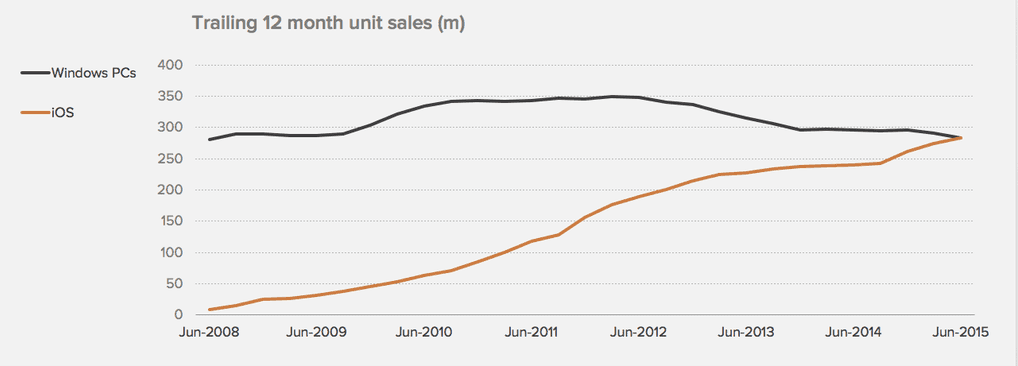
\includegraphics[width=150mm]{fig/ios_windows_compare}
  \caption{Сравнение объёма продаж устройств \\ под управлением iOS и Windows}
  \label{fig:ios_windows_compare}
\end{figure}

Из приведенного рисунка видно, что объём продаж устройств под управлением
iOS превысил продажи устройств под управлением OC Windows в июне 2015 года, а
годовые объемы продаж устройств на Android превысили ПК еще в марте 2012 года.
Количество действующих персональных компьютеров на платформе Windows оценивается
в 1,5 млрд устройств, объем работающих устройств на Android уже превысил этот
показатель, а iOS вполне может преодолеть аналогичный рубеж.

Мобильные устройства становятся удобнее для решения повседневных задач,
чем компьютеры. Этому служат следующие факторы:
\begin{itemize}
  \item низкая стоимость общения через мобильные устройства;
  \item использование сервисов геолокации;
  \item развитие сети LTE;
  \item тесное взаимодействие с пользователем.
\end{itemize}

Нативные приложения требуют установки и разрабатываются индивидуально
под мобильные платформы. И это их огромное преимущество перед web-приложениями.
Пользователь получает приятный внешний вид и бесперебойное
взаимодействие приложения с операционной системой устройства.
Такие приложения с наименьшими затратами используют камеру,
микрофон, акселерометр, плеер и прочие функции,
являясь наиболее безопасными и емкими.

По популярности мобильная операционная система iOS сильно уступает Android.
Между тем, главным преимуществом компании Apple является
состоятельность ее аудитории. При маленьком объеме рынка (около 12\%),
на устройства iOS приходится половина всех доходов
от продажи приложений --- \$6,4 млрд в год.
Кроме того, устройства Apple не так просто взломать.
Это еще одна причина высокой покупательской способности на платформе.

Отдельно стоит отметить, что по данным на январь 2016 года большинство
iOS (более 70\%) устройств используют
последнюю версию операционной системы от Apple, тогда как только 0,7\%
устройств на Android обновились до последней версии Android Marshmallow.
Диаграммы использования версий ОС представлены на рисунке~\ref{fig:ios_android_os_version}.

\begin{figure}[h!]
  \centering
  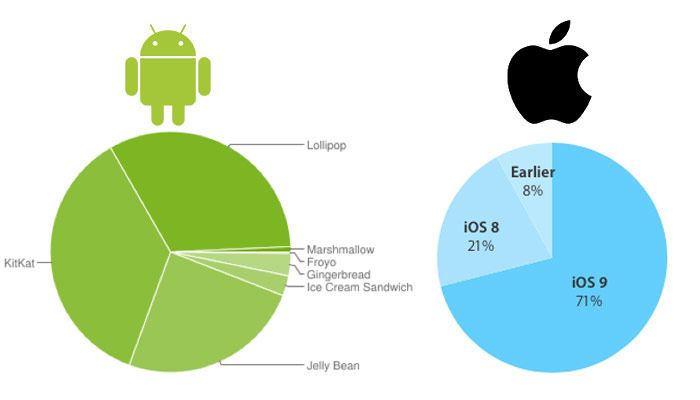
\includegraphics[width=150mm]{fig/ios_android_os_version}
  \caption{Использование версий ОС на мобильных устройствах \\ под управлением iOS и Android}
  \label{fig:ios_android_os_version}
\end{figure}

Сами разработчики мобильных приложений отдают предпочтение платформе Apple.
Отчасти это связано с тем, что при проектировании нужно учитывать всего
несколько форматов дисплеев. Возможно еще и потому,
что компания смогла упаковать инструменты разработки в более качественные
продукты, по сравнению с конкурентами~\cite{ios_android_compare}.

Учитывая то, что целевое назначение разрабатываемого продукта~--- предоставление
пользователю актуальной финансовой информации, то целесообразным является
разработать этот продукт в форм-факторе мобильного приложения. С этим связано
ряд дополнительных факторов:
\begin{itemize}
  \item разовая настройка приложения с учётом личных интересов;
  \item скорость доставки информации конечному пользователю;
  \item предоставление релевантной информации на основе данных,
    предоставляемых операционной системой.
\end{itemize}

Опираясь на достоинства операционной системы iOS, такие как защищенность
устройств, ограниченное количество размеров экранов, преобладание
использования последней версии операционной системы, а также большую, в сравнении
с другими мобильными платформами, состоятельность пользователей, в качестве
целевой мобильной платформы выберем операционную систему iOS, целевое устройство ---
iPhone.


\subsection{Сравнительный анализ существующих аналогов}

Рассмотрим наиболее популярные iOS приложения, позволяющие просматривать
информацию о курсах валют. Для этого воспользуемся магазином приложений от Apple,
введя в строке поиска запрос <<Курсы валют>>. В результате на выбор
пользователю будет представлено более десятка мобильных приложений в данной
категории. Учитывая то, в App Store используется достаточно
простой алгоритм формирования списка приложений, основанный прежде всего на
количестве скачиваний, можно утверждать, что первые приложения из этого списка
являются наиболее популярными. Рассмотрим первые пять приложений из этого
списка:
\begin{itemize}
  \item <<Курсы валют в Минске>> (Alex L);
  \item <<Курсы валют, банкоматы, обменники>> (Alex L);
  \item <<Финансы TUT.BY: курсы валют, конвертер>> (TUT.BY);
  \item <<Онлайнер - новости, курсы валют>> (Orangesoft LLC);
  \item <<Курс Валют Беларусь>> (Mobinovo).
\end{itemize}

Все приведенные приложения распространяются бесплатно, и только некоторые из
них включают <<встроенные покупки>>.

Для сравнения приложений будем использовать ряд критериев, которые условно
можно разделить на две группы: критерии функциональности и критерии удобства
использования.

Приложение <<Курс Валют Беларусь>> можно убрать из рассмотрения, так как оно
закрывается сразу после открытия (приложение принудительно завершается
стандартным обработчиком ошибок).

\newpage

Приведём критерии функциональности:
\begin{itemize}
  \item возможность отображения курсов валют в коммерческих банках;
  \item возможность отображения курсов валют, установленных национальным
    банком Республики Беларусь;
  \item наличие информации об отделениях банка;
  \item возможность отображения курсов валют в отделениях;
  \item возможность отображения отделения (банка) на карте;
  \item возможность поиска ближайших отделений (банков);
  \item отображение курсов валют в регионах;
  \item возможность отправки Push-уведомлений.
  \item возможность добавления отделений (банков) в избранное или закладки.
\end{itemize}

Критерии функциональности составлены с учётом основных возможностей
мобильных устройств, предоставляемой информации веб-ресурсами,
а также на основе изучения финансов порталов, предоставляющих пользователю
информацию о курсах валют.

Приведём критерии удобства использования:
\begin{itemize}
  \item стабильность работы приложения;
  \item простота восприятия информации;
  \item актуальность предоставляемой информации;
  \item дизайн (соответствие последней версии iOS);
  \item наличие рекламы;
\end{itemize}

Критерии удобства использования приложения сформированы на основе личного опыта
использования устройств под управлением операционной системы от Apple, а также
документа, содержащего рекомендации по разработке iOS приложений~---
iOS Human Interface Guidelines~\cite{ios_hig}.

Для получения максимально объективной оценки сравнительного анализа в перечень
критериев не будем включать какие-либо конкретные составляющие дизайна, например:
\begin{itemize}
  \item шрифт;
  \item размер текста;
  \item основная цветовая схема приложения;
\end{itemize}

Вместо этого, постараемся убедится в том, что рассматриваемые приложения
соответствует рекомендациям документа iOS Human Interface Guidelines.

\newpage

Произведем сравнение существующих аналогов по приведенным критериям. Для удобства
восприятия полученной информации, представим результаты сравнения в виде таблиц.
Результат сравнения по критериям функциональности представлен
в таблице~\ref{tbl:functionality_compare}.

\begin{table} [h!]
  \caption{
    Сравнение аналогов по критериям функциональности
  }\label{tbl:functionality_compare}
    \begin{tabular}{| m{8.5cm} | c | c | c | c |}
      \hline
      \parbox{7cm}{
        Критерий сравнения
      }
      & \rotatebox[origin=c]{90}{
          \parbox{4.2cm}{
            Курсы валют \\ в Минске
          }
        }
      & \rotatebox[origin=c]{90}{
          \parbox{4.2cm}{
            Курсы валют, \\ банкоматы, \\ обменники
          }
        }
      & \rotatebox[origin=c]{90}{
          \parbox{4.2cm}{
            Финансы TUT.BY: \\ курсы валют, \\ конвертер
          }
        }
      & \rotatebox[origin=c]{90}{
          \parbox{4.2cm}{
            Онлайнер -- \\ новости, \\ курсы валют
          }
        }
      \\
      \hline

      Отображение курсов валют \par в коммерческих банках
      & +
      & +
      & +
      & + \\
      \hline

      Отображение курсов валют \par национального банка РБ
      & +
      & +
      & +
      & + \\
      \hline

      Информация об отделениях банка
      & +
      & +
      & +
      & + \\
      \hline

      Отображение курсов валют \par в конкретных отделениях
      & -
      & -
      & +
      & + \\
      \hline

      Отображения отделений (банков) \par на карте
      & -
      & +
      & +
      & + \\
      \hline

      Поиск ближайших отделений \par (банков)
      & -
      & +
      & +
      & - \\
      \hline

      Отображение курсов валют \par в регионах
      & -
      & +
      & +
      & -  \\
      \hline

      Наличие Push-уведомлений
      & -
      & +
      & -
      & -  \\
      \hline

      Добавления отделений (банков) \par в избранное или закладки
      & -
      & +
      & -
      & -  \\
      \hline

    \end{tabular}
\end{table}

\newpage

Результат сравнения по критериям удобства использования представлен
в таблице~\ref{tbl:ux_compare}.

\begin{table} [h!]
  \caption{
    Сравнение аналогов по критериям удобства использования
  }\label{tbl:ux_compare}
    \begin{tabular}{| m{8.5cm} | c | c | c | c |}
      \hline
      \parbox{7cm}{
        Критерий сравнения
      }
      & \rotatebox[origin=c]{90}{
          \parbox{4.2cm}{
            Курсы валют \\ в Минске
          }
        }
      & \rotatebox[origin=c]{90}{
          \parbox{4.2cm}{
            Курсы валют, \\ банкоматы, \\ обменники
          }
        }
      & \rotatebox[origin=c]{90}{
          \parbox{4.2cm}{
            Финансы TUT.BY: \\ курсы валют, \\ конвертер
          }
        }
      & \rotatebox[origin=c]{90}{
          \parbox{4.2cm}{
            Онлайнер -- \\ новости, \\ курсы валют
          }
        }
      \\
      \hline

      Стабильность работы приложения
      & +
      & +
      & +
      & + \\
      \hline

      Простота восприятия информации
      & +
      & -
      & -
      & + \\
      \hline

      Актуальность предоставляемой \par информации
      & +
      & +
      & +
      & + \\
      \hline

      Дизайн (соответствие последней \par версии iOS 9)
      & +
      & -
      & +
      & + \\
      \hline

      Отсутствие рекламы
      & -
      & -
      & +
      & + \\
      \hline

    \end{tabular}
\end{table}

Из приведенной сравнительной характеристики видно, что каждое из приложений
обладает рядом достоинств, но вместе с тем, имеет и ряд недостатков.

Например, приложение <<Онлайнер -- новости, курсы валют>>, несмотря на высокие
показатели по критериям <<удобство использования>>, является, в первую очередь,
новостным приложением, и курсы валют предоставляет в качестве дополнительного сервиса.

В то же время приложение <<Курсы валют в Минске>>, несмотря на достаточно
ограниченную функциональность, является наиболее простыми в использовании, так как
предоставляет всю информацию о курсах валют на одном экране. Однако, если
пользователю требуется найти отделение банка на карте, то понадобится открывать
стороннее приложение, которое, в свою очередь, является очень перегруженным.

\newpage

В результате проведенного сравнения можно выделить приложение <<Курсы валют
в Минске>> и <<Финансы TUT.BY: курсы валют, конвертер>>. Оба эти приложения
соответствуют рекомендациям Apple по разработке мобильных приложений,
предоставляют актуальную информацию, но при этом обладают
разной функциональностью.
Снимки главных экранов приведенных приложений приведены на рисунке~\ref{fig:tutby_exchanges_minsk_screenshots}.

\begin{figure} [h]
  \begin{minipage} [h] {0.49\linewidth}
    \center{
      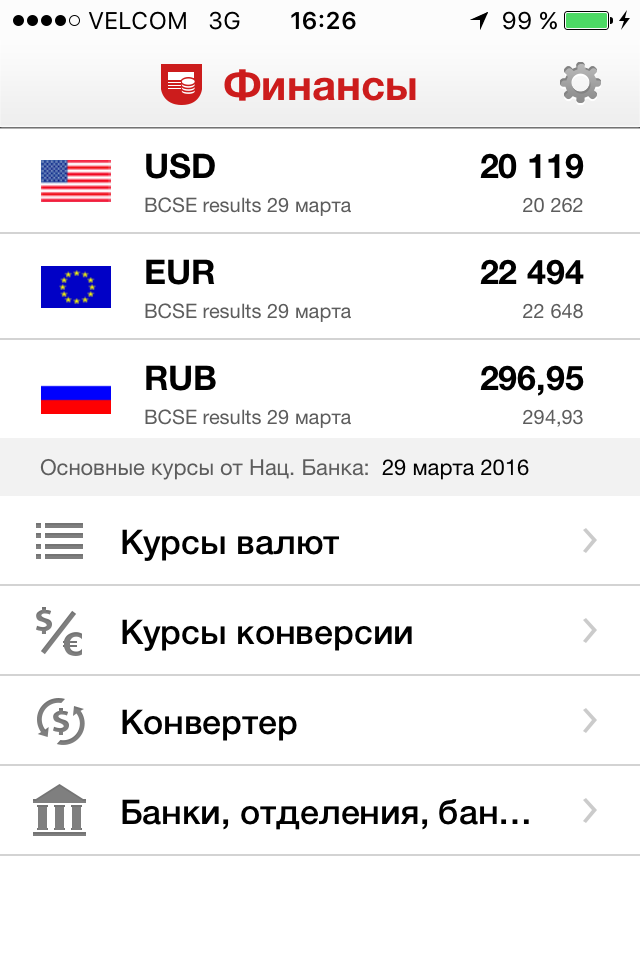
\includegraphics[width=0.85\linewidth]{fig/tut_by_screen}
    }
  \end{minipage}
  \hfill
  \begin{minipage} [h] {0.49\linewidth}
    \center{
      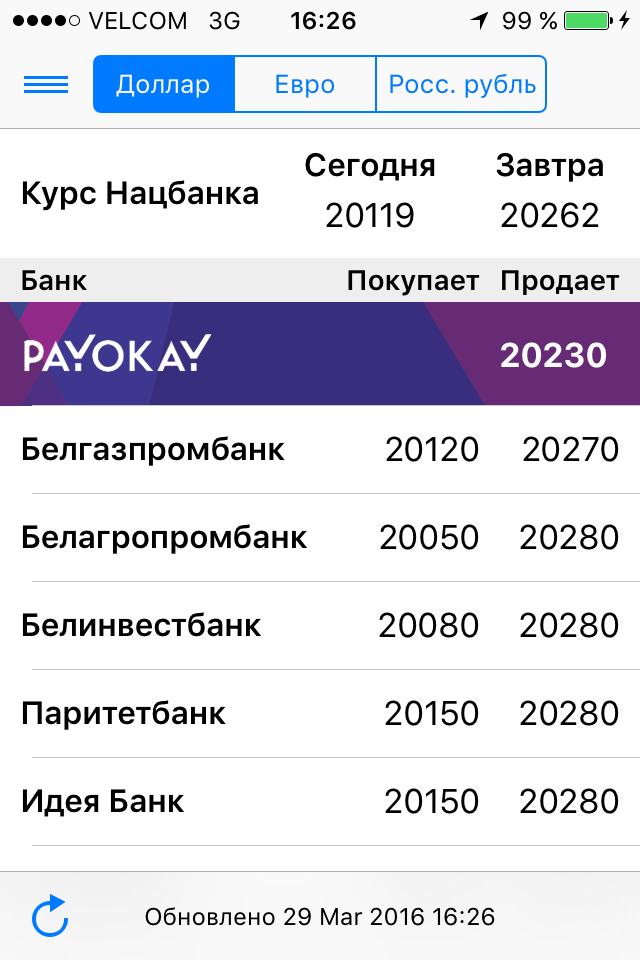
\includegraphics[width=0.85\linewidth]{fig/exchanges_minsk_screen}
      }
    \end{minipage}
  \caption{Снимки главных экранов приложений \\ <<Финансы TUT.BY>> и <<Курсы валют в Минске>>}
  \label{fig:tutby_exchanges_minsk_screenshots}
\end{figure}

Первое из приведенных приложений позволяет
максимально быстро узнать о курсе валют, а приложение от разработчика TUT.BY Media
предлагает за более длительное время получить гораздо больше информации.


\subsection{Обзор источников финансовой информации}

С учётом выбранной программной платформы, а также целевого назначения
разрабатываемого приложения стоит уделить внимание обзору источников
финансовой информации для приложения.

\newpage

Рассмотрим различные интернет-порталы, которые обладают финансовой информацией,
актуальной на территории Республики Беларусь. Вот некоторые из них:
\begin{itemize}
  \item select.by;
  \item finance.tut.by;
  \item myfin.by;
  \item vkurse.by;
  \item benefit.by;
  \item infobank.by;
  \item ecopress.by.
\end{itemize}

При рассмотрении порталов следует учитывать следующие критерии:
\begin{itemize}
  \item портал-первоисточник (из рассмотрения можно убрать порталы,
    которые не являются первоисточниками информации);
  \item отображение курсов валют в отделениях;
  \item наличие дополнительной информация об отделении;
  \item наличие прайс-листа на предоставление финансовой информации;
  \item наличие собственного мобильного приложения.
\end{itemize}

В результате из приведенных выше интернет-порталов для дальнейшего
рассмотрения можно оставить только некоторые из них select.by, myfin.by,
infobank.by, ecopress.by. Ни один из приведенных интернет-порталов не
предоставляет открытого API для доступа к курсам валют. Для того, чтобы определить,
кто может предоставить финансовые данные на безвозмездной основе, требуется
установить контакт с редакторами финансовых порталов. В результате
проделанной работы по поиску API с финансовыми данными выбор был сделан в
пользу финансового портала myfin.by.

Со стороны сервера (API myfin.by) предоставляется XML-файл, размер файла для
города Минска --- около 500 Кбайт.

Стоит заметить, что при использовании API сайта myfin.by напрямую, все
дополнительные вычисления необходимо будет выполнять на стороне клиента (iPhone).
Такой подход сильно противоречит рекомендациям Apple по разработке
мобильных приложений, в которых речь идёт об ограничении нагрузки на iOS
устройства.
К дополнительным вычислениям, связанным с обработкой полученных данных, можно отнести:
\begin{itemize}
  \item преобразование исходного XML файла в объекты модели;
  \item выбор лучшего курса;
  \item расчёт среднего курса;
  \item расчёт количества элементов;
  \item расчёт расстояния от устройства до отделений банков.
\end{itemize}

Учитывая то, что у разработчиков мобильного приложения нет возможности изменять
API сайта myfin.by или добавлять в него какие-либо функции, то целесообразным
является создание промежуточного сервера, который сможет выполнять некоторые
из приведенных операций, уменьшить количество выполняемых операций на стороне
клиента. Ещё одной положительной сторой использования промежуточного сервера
данных является возможность использовать иной формат передачи данных с
использованием компрессии, что может существенно сократить использование
интернет-трафика на мобильном устройстве.


\subsection{Постановка задачи проектирования}

С учётом выполненного анализа приложений-аналогов, а также полученного доступа к
API сайта myfin.by c данными о курсах валют, можно сформировать основные
требования к разрабатываемому приложению.

Требуется разработать мобильное iOS приложение, позволяющее пользователям
просматривать актуальные курсы валют в отделениях коммерческих банков, а также
установленные национальном банком Республики Беларусь. С использованием
служб геолокации дать пользователям возможность находить ближайшие отделения,
просматривать детальную информацию об этом отделении, просматривать отделения
на карте. Достаточно широкая функциональность приложения не должна перегружать
интерфейс пользователя. Должна быть предусмотрена работа приложения в
оффлайн-режиме (сохранение финансовой информации в локальную базу данных).
Разработанное приложение должно соответствовать рекомендациям по созданию
iOS приложений от Apple, приведенных в iOS Human Interface Guidelines.

\pagebreak
